% this file is called up by thesis.tex
% content in this file will be fed into the main document
\chapter{Regiones Ionizadas}



\lettrine[lines=1]{A}unque es un trabajo sobre poblaciones estelares, es interesante saber por que consideramos a UGC11680 como una galaxia espiral con un AGN  tipo 2. Este tipo de análisis se puede realizar ya sea con cada espectro de las galaxias de la muestra o espectros integrados para resultados estadísticos. Este proceso se  hace con las líneas de emisión de cada espectro de la galaxia, lo cual hacemos un breve resumen del análisis realizado, para ver que es así.


\begin{figure}[!ht]
  \centering
  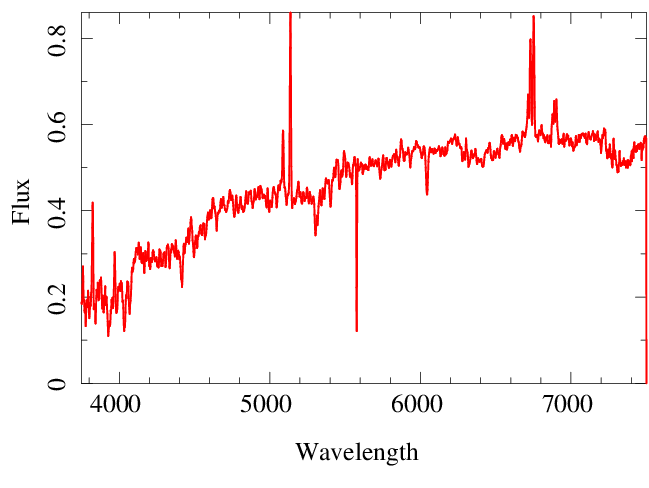
\includegraphics[width=4in]{spec_cen_UGC11680NED01.png}
  \caption[Espectro central UGC11680]
   {Espectro en el óptico de la region central de UGC11680 sacado directamente de su cubo de datos, en \textbf{CALIFA}. Las longitudes de onda están en sus valores en el marco de referencia del laboratorio. Notese la ausencia de componentes de líneas anchas y las líneas prohibidas del oxígeno ([O III] $\lambda \lambda$4959, 5007 \text{\AA}, [O I] $\lambda$6300 \text{\AA}), y las líneas de  nitrógeno ([N II]  $\lambda \lambda$ 6548, 6583 \text{\AA}), y silicon ([S II] $\lambda \lambda$6716, 6731 \text{\AA}), características de un AGN tipo II.  Nótese que la linea de  [N II] esta casi mezclada con  $H_{\alpha}$ en $\lambda$ = 6563 \text{\AA} }
\label{espectro}
\end{figure}


\begin{figure}[!ht]
  \centering
  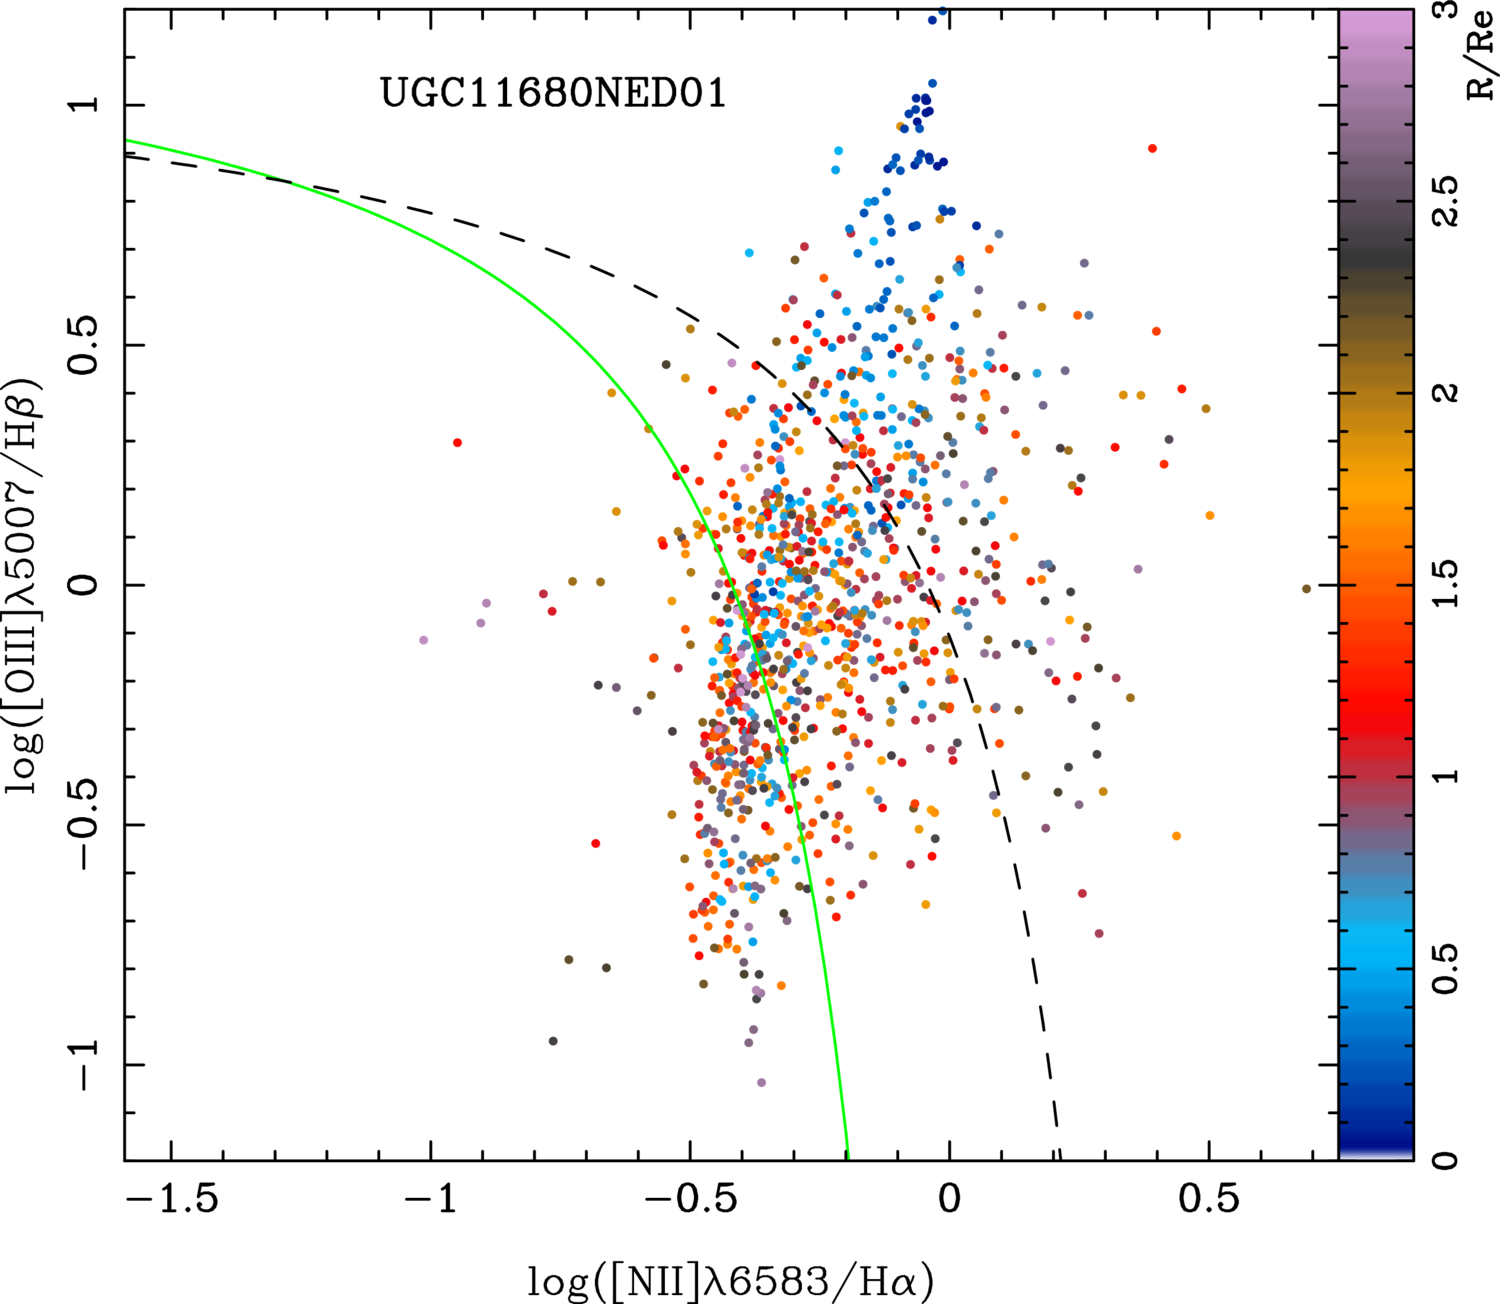
\includegraphics[scale=0.2]{1UGC11680NED01_proc_elines4.png}
  \caption[ Diagrama bpt UGC11680]
   {Diagrama BPT de  UGC11680,usando las líneas ya corregidas de [O III]$\lambda$5007/$H_{\beta}$ vs.
[N II]$\lambda$6583/$H_{\alpha}$. Los puntos azules indican zonas galactrocentricas amarillas a rojas la zona media y moradas las afueras. La line solida representa un modelo de region HII la linea punteada, conocida como la línea de ``Kewley'' divide la ionización por AGN de las zonas ionizadas por regiones HII, mientras que la linea verde denota la linea de  ``Kauffmann''. Obsérvese que a pesar de la ionización del AGN, UGC11680 sigue mostrando regiones HII y por lo tanto formación estelar en sus afueras. }
\label{bpt}
\end{figure}


\section{Diagramas BPT}

\bigskip

Tras el descubrimiento de galaxias espirales con un núcleo muy brillante que emite
(líneas de emisión de varios miles de km/s) (\citet{seyfert1941}),
se hizo evidente que estos núcleos galácticos eran el lugar de una violenta,
actividad no estelar (\citet{burbidge1963}), tal vez de la misma naturaleza que se encontró en los cuásares.
Heckman  realizó un análisis espectroscópico de los núcleos de una muestra completa
de 90 galaxias, y  encontró que la presencia de baja ionización nuclear (LINERS) eran bastante comunes, y parecían ser
la versión reducida de los núcleos Seyfert. \cite{baldwin1981} fueron los
primero en proponer diagnósticos espectroscópicos sobre la base de relaciones de línea de emisión
para distinguir galaxias normales  de formación estelar de los AGNs. El más famoso es el que compara los cocientes de líneas
[O III] $\lambda$5007/$H_{\beta}$ vs [N II]$\lambda$6583/$H_{\alpha}$ a menudo referido como el diagrama de BPT (por Baldwin, Phillips,
Y Terlevich).

\bigskip

\noindent \citet{osterbrock1987} propusieron diagramas adicionales: [O III] $\lambda$5007/$H_{\beta}$ vs
[S II] $\lambda$6725 /$H_{\alpha}$, y [O III] $\lambda$5007/$H_{\beta}$ vs [S i] $\lambda$6300/$H_{\alpha}$.
Como es conocido \citet{osterbrock1989}, las regiones H II  forman una
secuencia mas estrecha en estos diagramas. Sólo unos años después, \citet{kewley2001}  construyeron un \textsl{grid} de
modelos de fotoionización a fin de determinar un límite superior teórico
a la ionización por las estrellas masivas en el diagrama de BPT. Este límite superior,
más adelante se hace referencia como la ``línea de Kewley". \citet{kauffmann2003} desplazaron esta línea a la izquierda para definir un límite empírica entre galaxias normales de formación de estrellas y que tienen un AGN (la línea de ``Kauffmann")

\bigskip

\noindent De esta forma,Como tenemos un ejemplo típico de una galaxia  con resolución espacial, podemos hacer un diagrama BPT sólo para una galaxia y por lo tanto cada punto representa un zona en nuestra galaxia. La figura \ref{bpt} representa
la gráfica de [O III] $\lambda$5007/$H_{\beta}$ vs [N II]$\lambda$6584/$H_{\alpha}$ de un diagrama BPT para UGC11680.
En este gráfico podemos ver dos líneas curvas diferentes. Los puntos por encima y a la derecha de la línea de puntos representa
zonas ionizadas por el AGN, mientras que los puntos de abajo y hacia la izquierda para
la línea de trazos representan zonas de formación de estrellas. Los
puntos en el medio representan zonas que tienen características
de ambas regiones ionizadas por AGN  y de formación de estrellas HII. Observamos entonces que para UGC11680 las regiones centrales, se encuentran ionizadas por procesos no estelares, lo que puede ser la presencia de un AGN. Obsérvese también que esta galaxia tiene presencia de regiones HII en las afueras, lo que implica que esta galaxia sigue formando estrellas.

\bigskip

\noindent Resumiendo, el espectro de la zona central, así como su diagrama BPT, nos indican que UGC11680 es una galaxia con AGN tipo II, y que a pesar de no ser notorio en sus imágenes en el óptico, esta galaxia sigue formando estrellas aunque a una tasa baja, debido a la presencia de regiones HII en las zonas exteriores dadas por el radio efectivo. Este resultado,coincide con los resultados que se obtuvieron por análisis de poblaciones estelares, es decir, aunque la galaxia tiene un color rojo en el óptico, esta sigue formando estrellas, aunque a una tasa baja.

\chapter{Tabla de conversión}

\begin{table}[!ht]
\centering
\begin{tabular}{||c | c | c||}
\hline
\hline
Look back in time (Gyrs) & Edad (Gyrs) & $\sim$ redshift $z$ \\
\hline
\hline


1.122  & 13.0  & 0.070  \\
1.259 & 12.8 & 0.080   \\
1.42  & 12.2 & 0.083  \\
2.0  & 11.8 & 0.15  \\
2.5 & 11.4 & 0.19  \\
3.55  & 10.6 & 0.3  \\
4.5  & 9.4 & 0.4  \\
6.3 & 8.4 & 0.65  \\
8.0   &  6.2 & 0.8  \\
10.0  & 4.1  & 1.7  \\
12.6  & 1.5  & 4.7  \\
14.2  & 0.1  & 19  \\

\hline
\hline
\end{tabular}
\caption{Tabla de conversión entre edades para el estudio de la historia de formación estelar usada en la tesis asi como su aproximación en redshift $z$, usando los datos cosmologicos $\Omega_m = 0.317$ , $\Omega_{\Lambda}=0.683$ y $H_0 = 67.15$ km/s/Mpc \citep{plank2014}} 
\label{tab_conversion}                              %etiqueta para referencia
\end{table}
